\documentclass[12pt]{article}
\usepackage{geometry}                % See geometry.pdf to learn the layout options. There are lots.
\geometry{letterpaper}                   % ... or a4paper or a5paper or ... 
%\geometry{landscape}                % Activate for for rotated page geometry
\usepackage[parfill]{parskip}    % Activate to begin paragraphs with an empty line rather than an indent
\usepackage{daves,fancyhdr,natbib,graphicx,dcolumn,amsmath,lastpage,url}
\usepackage{amsmath,amssymb,epstopdf,longtable}
\usepackage{paralist}  % need to modify standard enumerate blocks
\usepackage[final]{pdfpages}
\DeclareGraphicsRule{.tif}{png}{.png}{`convert #1 `dirname #1`/`basename #1 .tif`.png}
\pagestyle{fancy}
\lhead{CE 3354 -- Engineering Hydrology}
\rhead{SUMMER 2025}
\lfoot{ES2}
\cfoot{}
\rfoot{Page \thepage\ of \pageref{LastPage}}
\renewcommand\headrulewidth{0pt}

\begin{document}
\begin{center}
{\textbf{{ CE 3354 Engineering Hydrology} \\ {Exercise Set 2}}}
\end{center}

\section*{\small{Exercises}}
\begin{enumerate}
\item A raingage is located in a 2.5 acre impervious watershed with non initial abstraction.  The gage records a catch of 1.0 inches of precipitation in one hour.  The maximum intensity was 2.4 inches per hour for 10 minutes.  Assume that 10 minutes is the characteristic time for which all parts of the watershed can contribute runoff to a discharge point.

Determine:
    \begin{enumerate}[a)]
        \item Volume of rainfall in cubic feet for the watershed. 
        \item Maximum (peak) discharge rate for the watershed.
    \end{enumerate}

Solution(s):


\begin{enumerate}[a)]
\item Find volume of rainfall in cubic feet as product to total depth and wassershed area.
\begin{equation}
V=A \times\ D = 2.5~ac \cdot \frac{43560~ft^2}{1~ac} \cdot 1.0~in \cdot \frac{1~ft}{12~in} = 9,074~ft^3
\end{equation}
\item Apply rational runoff equation to estimate peak discharge.

\begin{equation}
Q_{peak} = C \cdot i\cdot A = (1.0)(2.4)(2.5) = 6.0~cfs
\end{equation}

Where:\\
Q = peak discharge in cfs\\
C = runoff coefficient (1.0 for impervious surfaces, given)\\
i = rainfall intensity (2.4 in/hr, given maximum 10-min intensity) for the time of concentration (10 minutes, given)\\
A = area in acres (2.5 ac., given)\\

\end{enumerate}

\clearpage

\item Consider the rainfall data in Table \ref{tab:SomewhereUSARain}

\begin{table}[h!]
\centering
\caption{Somewhere USA Precipitation Data}
\begin{tabular}{p{2.0in}p{2.0in}} % Column formatting, @{} suppresses leading/trailing space
~&~\\
Time (minutes) & Cumulative Depth (inches\\
\hline
\hline
0.00 & 0.00 \\
30.0 & 0.04 \\
60.0 & 0.38 \\
90.0 & 1.07 \\
120. & 1.44 \\
150. & 1.62 \\
180. & 1.70 \\
\hline
\end{tabular}
\label{tab:SomewhereUSARain}
\end{table}

Determine:
    \begin{enumerate}[a)]
        \item A depth (cumulative inches) hyetograph in 30 minute intervals (plot). 
        \item An intensity (inches/hour) hyetograph in 30 minute intervals (plot).
    \end{enumerate}

Solution(s):
Both items above are shown on Figure \ref{fig:es2-2}

\begin{figure}[h!] %  figure placement: here, top, bottom, or page
   \centering
   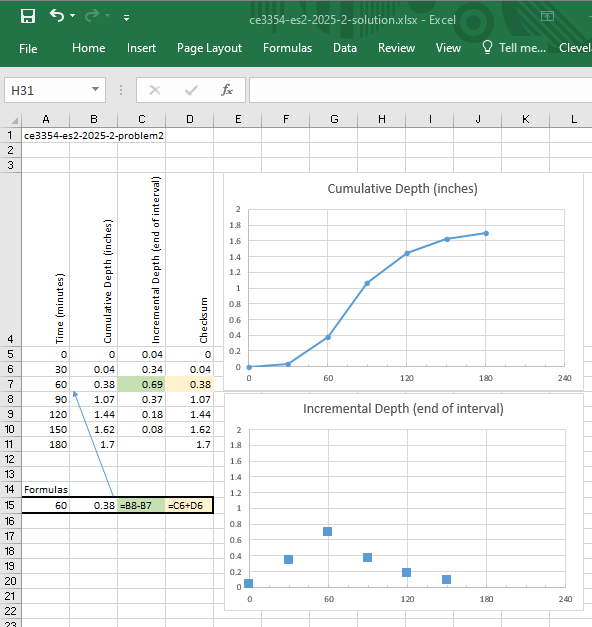
\includegraphics[height=3in]{ES2-2.png} 
   \caption{Excel screen capture for ES2-2 (both parts)}
   \label{fig:es2-2}
\end{figure}

\clearpage
%%%%%%%%%%%%%%%%%%%%%%%%%%%%%%%%%%%%%%%%%%%%%%%%%%%%

\item The intersection of US 408 and US 417 in Orange County, Florida at 28°32'51.2"N 81°15'28.5"W is the approximate centroid of that county. Using NOAA Atlas 14 (use the online PFDS tool)

Determine:
    \begin{enumerate}[a)]
        \item The 1-hr rainfall depth for a 100-yr Annual Recurrance Interval (ARI). 
        \item The 1-hr average rainfall intensity for a 100-yr Annual Recurrance Interval (ARI). 
        \item The 6-hr rainfall depth for a 100-yr Annual Recurrance Interval (ARI). 
        \item The 6-hr average rainfall intensity for a 100-yr Annual Recurrance Interval (ARI). 
    \end{enumerate}

Solutions:

\begin{figure}[h!] %  figure placement: here, top, bottom, or page
   \centering
   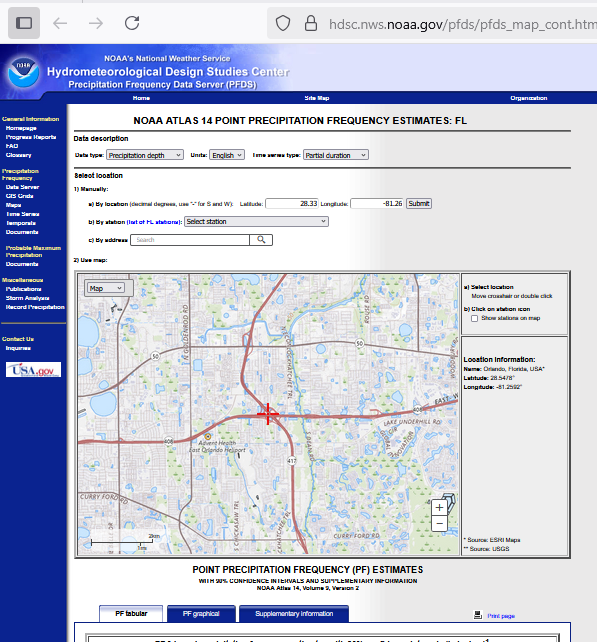
\includegraphics[height=5in]{pfds-1.png} 
   \caption{NOAA PFDS Locating the place of interest}
   \label{fig:pfds-1}
\end{figure}

\begin{figure}[h!] %  figure placement: here, top, bottom, or page
   \centering
   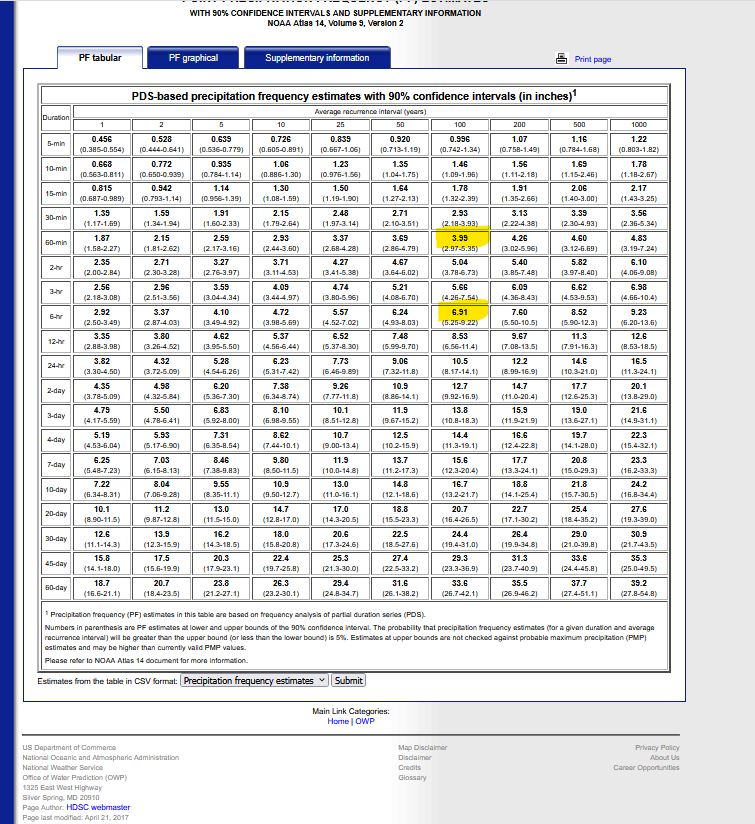
\includegraphics[height=5in]{pfds-2.png} 
   \caption{Depth for different reurrance intervals}
   \label{fig:pfds-2}
\end{figure}

\begin{figure}[h!] %  figure placement: here, top, bottom, or page
   \centering
   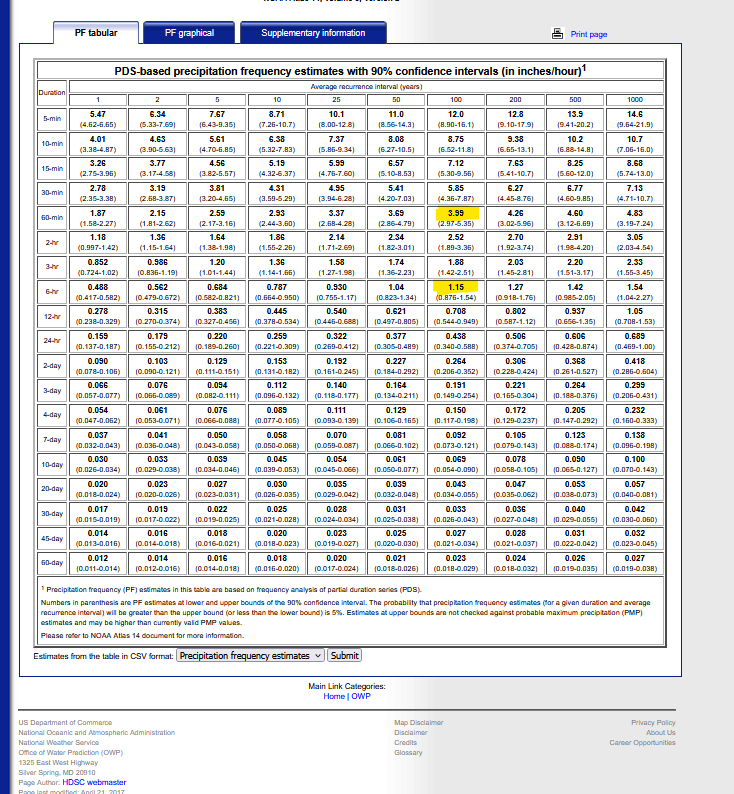
\includegraphics[height=5in]{pfds-3.png} 
   \caption{Intensity for different recurrance intervals}
   \label{fig:pfds-3}
\end{figure}
\clearpage
%%%%%%%%%%%%%%%%%%%%%%%%%%%%%%%%%%%%
\begin{table}[h!]
\centering
\caption{Summary Florida Depths and Intensity for the intersection of US 408 and US 417 in Orange County, Florida}
\begin{tabular}{p{2.0in}p{2.0in}p{2.0in}} % Column formatting, @{} suppresses leading/trailing space
~&~\\
Duration (hours) & Value & ARI (years)\\
\hline
\hline
1.0 & 3.55 inches & 100\\
1.0 & 3.55 inches/hour & 100 \\
6.0 & 6.91 inches & 100\\
6.0 & 1.15 inches/hour & 100\\
\hline
\end{tabular}
\label{tab:FloridaRainIDF}
\end{table}

\clearpage
%%%%%%%%%%%%%%%%%%%%%%%%%%%%%%%%%%%%%%%%%%%%%%%%%%%%%%%%%%%%%%%%%%%%%%%%%%

\item 55 mm of rain is recorded for a 6-hour storm by a raingage for a 10 km$^2$ watershed.  The runoff from the storm indicates that only 45 mm of rain fell on the entire area.  

    \begin{enumerate}[a)]
        \item The areal reduction factor  (ARF). 
        \item Compare the result to Central Texas areal reduction factors 
    \end{enumerate}

Solution(s):

Figure \ref{fig:ARFsoln}

\begin{figure}[h!] %  figure placement: here, top, bottom, or page
   \centering
   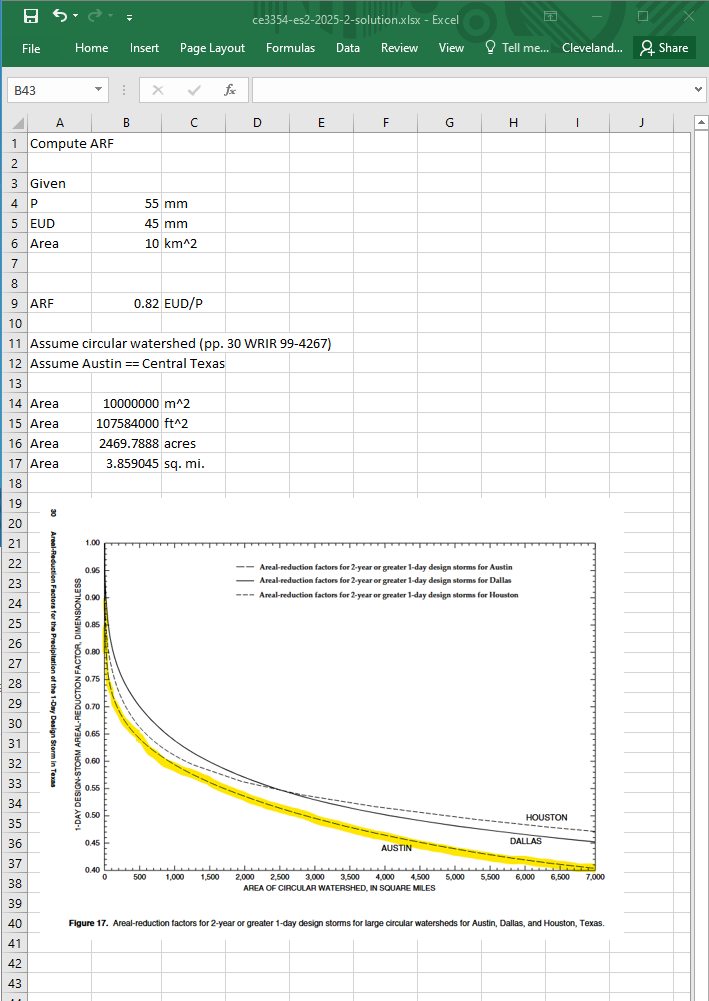
\includegraphics[height=5in]{ES2-4.png} 
   \caption{ARF computation and comparison to Central Texas}
   \label{fig:ARFsoln}
\end{figure}

The reported ARF is consistent with plotted ARF for the Austin curve, but the reported is smaller than anticipated with Central Texas behavior.

\clearpage
%%%%%%%%%%%%%%%%%%%%%%%%%%%%%%%%%%%%%%%%%%%%%%%%%%%%%%%%%%%%%%%%%%%%%%%%%%%%%%%
\item Table \ref{tab:SomewhereElseUSARain} is precipitation data for a 6-hour storm in Somewhere Else USA.

\begin{table}[h!]
\centering
\caption{Somewhere Else USA Precipitation Data -- End of Interval Catch}
\begin{tabular}{p{2.0in}p{2.0in}} % Column formatting, @{} suppresses leading/trailing space
~&~\\
Time (hours) & Cumulative Depth (inches\\
\hline
\hline
0.00 & 0.00 \\
0.25 & 0.10 \\
0.50 & 0.21 \\
0.75 & 0.33 \\
1.00 & 0.48 \\
1.25 & 0.64 \\
1.50 & 0.81 \\
1.75 & 1.08 \\
2.00 & 1.38 \\
2.25 & 2.46 \\
2.50 & 3.60 \\
2.75 & 3.90 \\
3.00 & 4.20 \\
3.25 & 4.44 \\
3.50 & 4.68 \\
3.75 & 4.86 \\
4.00 & 5.01 \\
4.25 & 5.16 \\
4.50 & 5.28 \\
4.75 & 5.40 \\
5.00 & 5.52 \\
5.25 & 5.64 \\
5.50 & 5.76 \\
5.75 & 5.88 \\
6.00 & 6.00 \\
\hline
\end{tabular}
\label{tab:SomewhereElseUSARain}
\end{table}

Determine:
    \begin{enumerate}[a)]
        \item The average rainfall intensity (inches/hour) from hour 3:00 to hour 4:00. 
        \item The average rainfall intensity (inches/hour) for the first half of the storm. 
        \item The maximum rainfall intensity (inches/hour) in any one hour.  
        \item The maximum rainfall intensity (inches/hour) in any 15-minute interval. 
        \item The average rainfall intens10ity (inches/hour) for the last half hour of the storm.   
    \end{enumerate}

Solution(s):

Figure \ref{fig:es2-5} is a screen capture with the various storm values; formulas used are shown in the figure.

\begin{figure}[h!] %  figure placement: here, top, bottom, or page
   \centering
   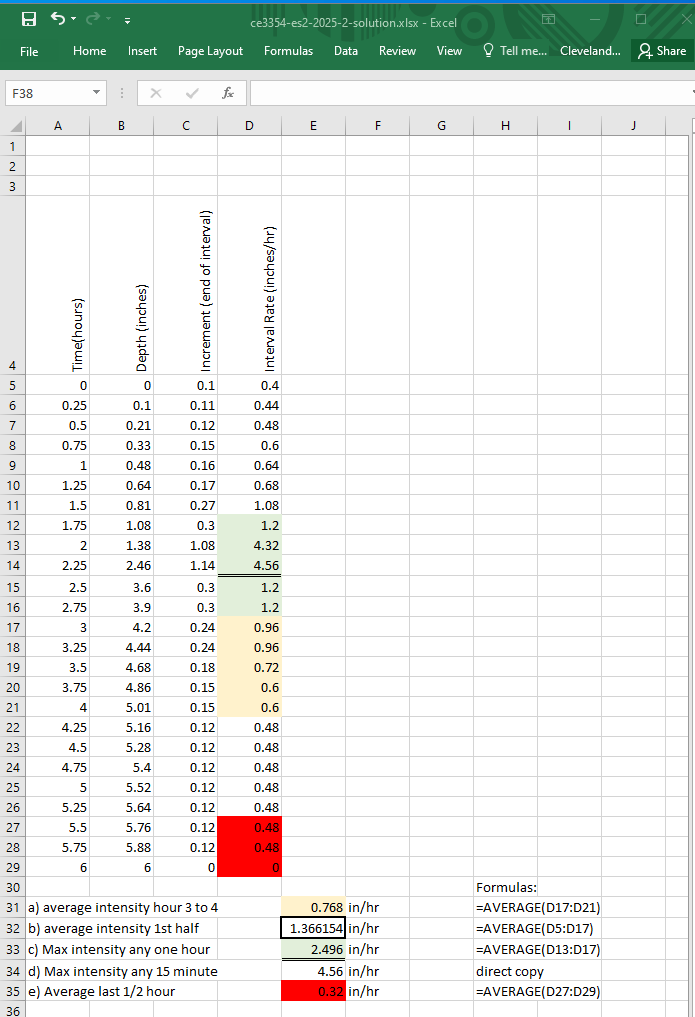
\includegraphics[height=5in]{ES2-5.png} 
   \caption{Various storm averages from Somewhere Else USA}
   \label{fig:es2-5}
\end{figure}

\clearpage

\item Using the NRCS Type III rainfall distribution

Determine:
    \begin{enumerate}[a)]
        \item The cumulative rainfall depth (inches) for half-hour increments for a 10 inch total depth, 24-hour storm.
        \item The rainfall intensity (inches/hour) for each half-hour increment of the storm. 
        \item The maximum rainfall intensity (inches/hour) in any 30-minute interval.  
    \end{enumerate}

Solution(s):

The python script below should interpolate the hyetographs onto the desired 15-minute space.  
Copy the output file into an Excel spreadsheet, and complete the exercise.

\begin{verbatim}
# Script to generate 1-minute hyetographs
import numpy as np
import pandas as pd
import matplotlib.pyplot as plt
from scipy.interpolate import interp1d
hyetType = 'type3'
PT = 1.0 # total depth - change to suit problem
#######################################
hour = [0,2,4,6,7,8,8.5,9,9.5,9.75,10,10.5,11,11.5,11.75,12,12.5,13.0,13.6,14,16,20,24,48]
minutes = [i*60 for i in hour]
hyets = {
        'type1': [0,0.035,0.076,0.125,0.156,0.194,0.219,0.254,0.303,0.362,
        0.515,0.583,0.624,0.654,0.669,0.682,0.706,0.727,0.748,0.767,0.83,0.926,1,1],
        'type1A': [0,0.05,0.116,0.206,0.268,0.425,0.48,0.52,0.55,0.564,0.577,
        0.601,0.624,0.645,0.655,0.664,0.683,0.701,0.719,0.736,0.8,0.906,1,1],
        'type2': [0,0.022,0.048,0.08,0.098,0.12,0.133,0.147,0.163,0.172,0.181,
        0.204,0.235,0.283,0.357,0.663,0.735,0.772,0.799,0.82,0.88,0.952,1,1],
        'type3': [0,0.02,0.043,0.072,0.089,0.115,0.13,0.148,0.167,0.178,0.189,
        0.216,0.25,0.298,0.339,0.5,0.702,0.751,0.785,0.811,0.886,0.957,1,1],
        'user': [0,0,0.4285,0.8571,1.0,1.0,1.0,1.0]  # Adjust time scaling below if needed
    }
if hyetType == 'user':
    user_time = [0,7,8,9,9.3333,10,24,48]
    minutes = [i*60 for i in user_time]
    hyet = hyets['user']
else:
    hyet = hyets.get(hyetType)
f = interp1d(minutes, hyet, kind='linear')
t24 = np.arange(0, 1455)  # 48 hours in minutes
depth = PT * f(t24)  # Scaled cumulative rainfall depth
intensity = np.diff(np.insert(depth, 0, 0)) * 60  # in/hr
# Build DataFrame ########################################
df = pd.DataFrame({
    "Time (min)": t24,
    "Cumulative Depth (in)": depth,
    "Intensity (in/hr)": intensity
})
# Optionally, write every nth row (e.g., every 15 minutes)
n = 15
df_thinned = df.iloc[::n]
# Save to CSV ##########################################################
df_thinned.to_csv(f"interpolated_output_{hyetType.upper()}.csv", index=False)
##########################################################################
\end{verbatim}

Figures \ref{fig:es2-6-xls} and \ref{fig:es2-6-form} are spreadsheet fragments to illustrate the building of the tool. Once the tool(s) are built simply query arrays as needed to complete the exercise.

\begin{figure}[h!] %  figure placement: here, top, bottom, or page
   \centering
   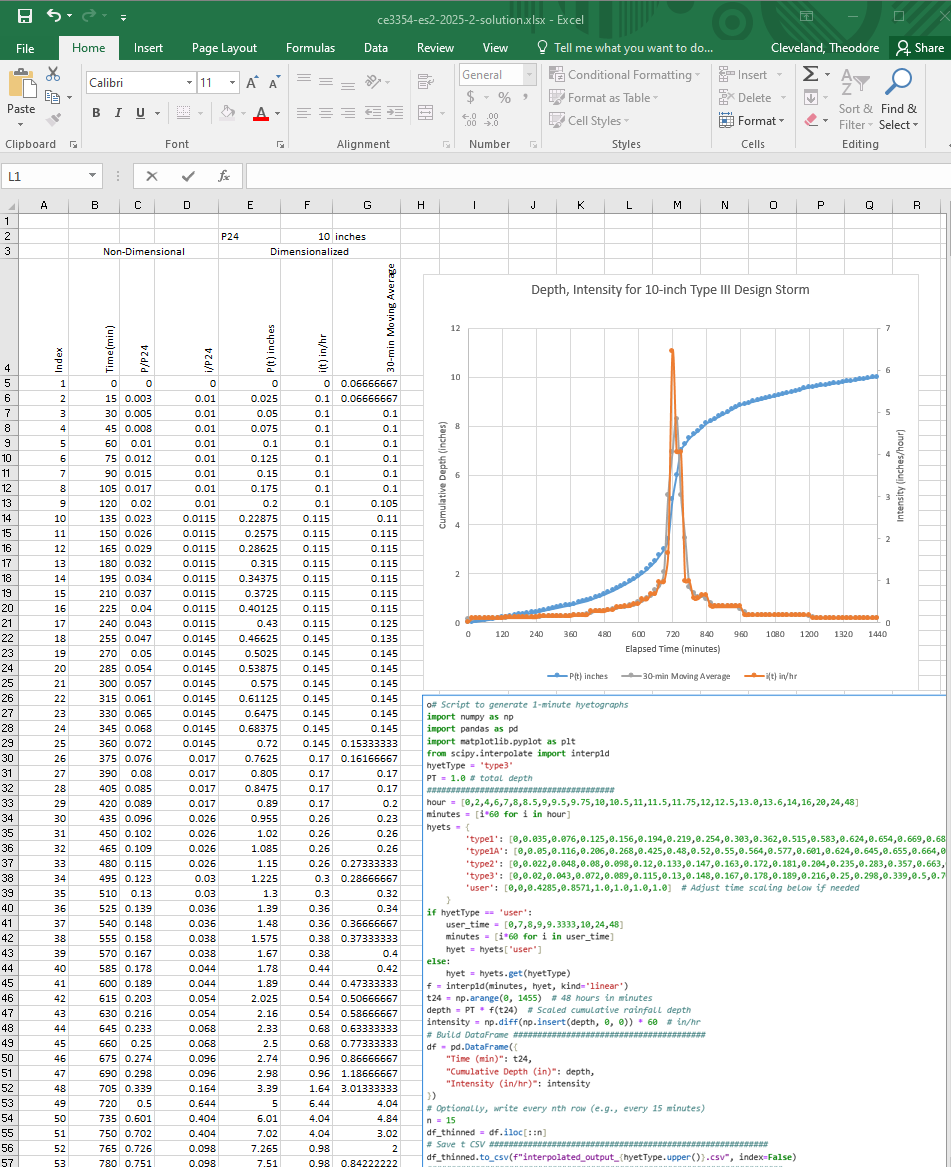
\includegraphics[height=6in]{ES2-6-xls.png} 
   \caption{Type III Storm Spreadsheet}
   \label{fig:es2-6-xls}
\end{figure}

\clearpage

\begin{figure}[h!] %  figure placement: here, top, bottom, or page
   \centering
   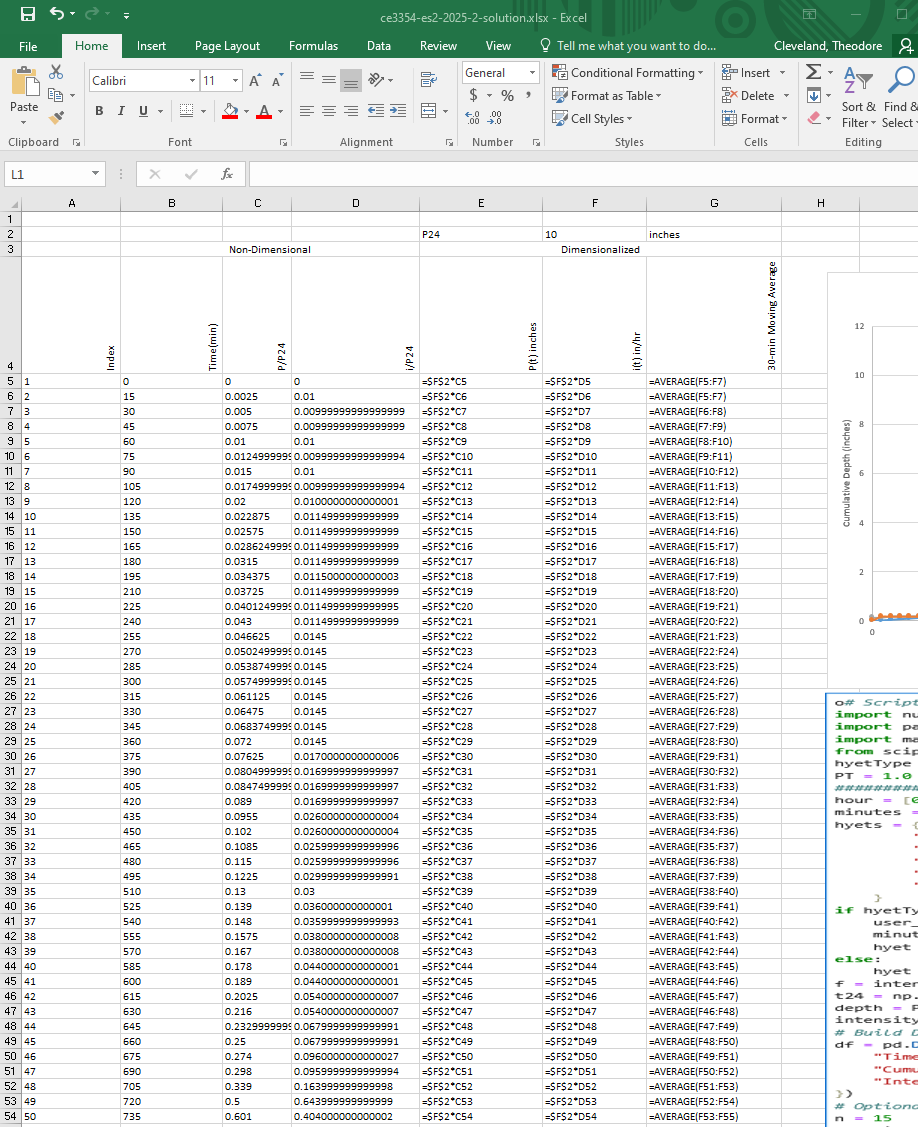
\includegraphics[height=6in]{ES2-6-formulas.png} 
   \caption{Type III Storm Spreadsheet (as formulas)}
   \label{fig:es2-6-form}
\end{figure}
\clearpage

\begin{enumerate}[a)]
        \item The cumulative rainfall depth (inches) for half-hour increments for a 10 inch total depth, 24-hour storm. The column labeled \textbf{P(t) inches} is the cumulative depth for the design storm.
        \item The rainfall intensity (inches/hour) for each half-hour increment of the storm. The column labeled \textbf{i(t) in/hr} is the intensity for the design storm.
        \item The maximum rainfall intensity (inches/hour) in any 30-minute interval.  The largest average of any 3 three adjacent rows would be the maximum 30-minute intensity.  In the image its the column labeled 30-minute moving average.  The largest value is 4.84 in/hr at time 735 minutes.(12:15 from the storm start)
    \end{enumerate}


\clearpage
%%%%%%%%%%%%%%%%%%%%%%%%%%%%%%%%%%%%%%%%%%%%%%%%%%%


\item Table \ref{tab:SomewhereUSARainIDF} is intensity duration data for Somewhere USA.

\begin{table}[h!]
\centering
\caption{Somewhere USA Intensity-Duration}
\begin{tabular}{p{2.0in}p{2.0in}} % Column formatting, @{} suppresses leading/trailing space
~&~\\
Duration (minutes) & Intensity (inches/hour) \\
\hline
\hline
10.0 & 4.00 \\
15.0 & 3.20 \\
20.0 & 2.70 \\
30.0 & 1.90 \\
60.0 & 1.20 \\
120. & 0.80 \\
180. & 0.60 \\
\hline
\end{tabular}
\label{tab:SomewhereUSARainIDF}
\end{table}

Determine:
    \begin{enumerate}[a)]
        \item Plot the intensity duration on the plot type that produces a straight line.
        \item An equation (model) of the "best" straight line for these values. 
    \end{enumerate}

Solution(s):

The attached spreadsheet in Figure \ref{fig:es2-7xls} shows the analysis.  

\begin{figure}[h!] %  figure placement: here, top, bottom, or page
   \centering
   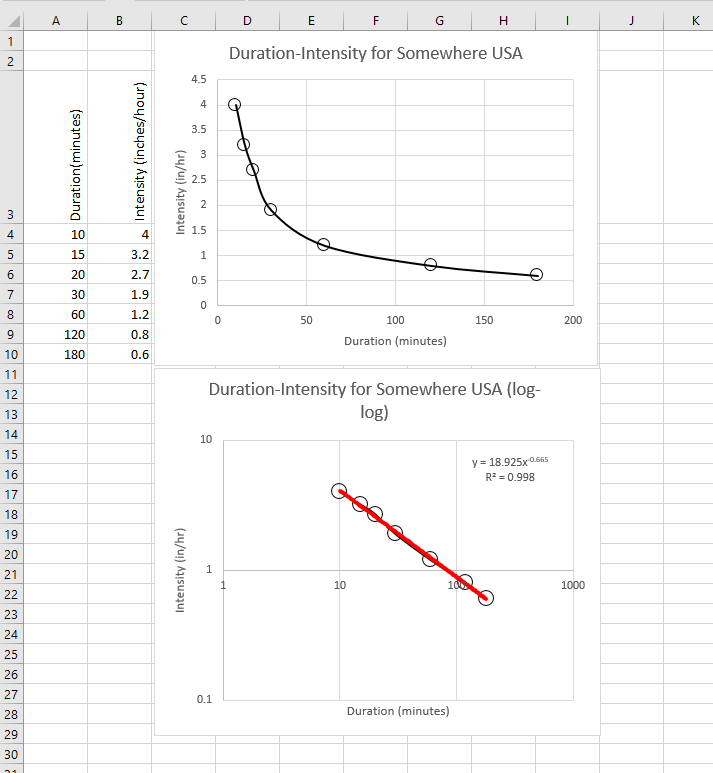
\includegraphics[height=4in]{es2-7xls.png} 
   \caption{Spreadsheet screen capture with arithmetic and double log plots.}
   \label{fig:es2-7xls}
\end{figure}

In this case the data, when plotted on log-log axes, align closely along a straight line. This suggests that the relationship between variables follows a power-law form of the type:

$ y=ax^b$
 
In a log-log plot, such relationships appear linear because:


$log(y)=log(a)+b \cdot log(x)$

This linearity in the transformed space indicates that a power-law model may be the most appropriate choice for describing the underlying behavior of the data.

The equation based on the plot (using Excel Trendline) is
\begin{equation}
I_{in/hr} = 18.925 \cdot T_{c~min}^{0.665}
\end{equation}

\clearpage

\item Table \ref{tab:Baltimore} is a measured 1-hour hyetograph for Baltimore, Maryland.

\begin{table}[h!]
\centering
\caption{Baltimore, Maryland Rainfall Data}
\begin{tabular}{p{2.0in}p{2.0in}} % Column formatting, @{} suppresses leading/trailing space
~&~\\
Time (minutes) & Intensity (cm/hour) \\
\hline
\hline
0.00 - 10.0 & 2.00 \\
10.0 - 20.0 & 6.00 \\
20.0 - 30.0 & 12.00 \\
30.0 - 40.0 & 8.00 \\
40.0 - 50.0 & 6.00 \\
50.0 - 60.0 & 3.00 \\
\hline
\end{tabular}
\label{tab:Baltimore}
\end{table}

Determine:
    \begin{enumerate}[a)]
        \item The average intensity in cm/hr.
        \item The net volume of rainfall in m$^3$ and liters if the watershed is 4,000 m$^2$
        \item An approximate Annual Recurrance Interval (ARI) for the measured event, using NOAA Atlas 14. 
    \end{enumerate}

Solution(s):

a), b), and c) are shown in the spreadsheet in Figure \ref{fig:es2-8xls} and the formulas used are in Figure \ref{fig:es2-8func}

\begin{figure}[h!] %  figure placement: here, top, bottom, or page
   \centering
   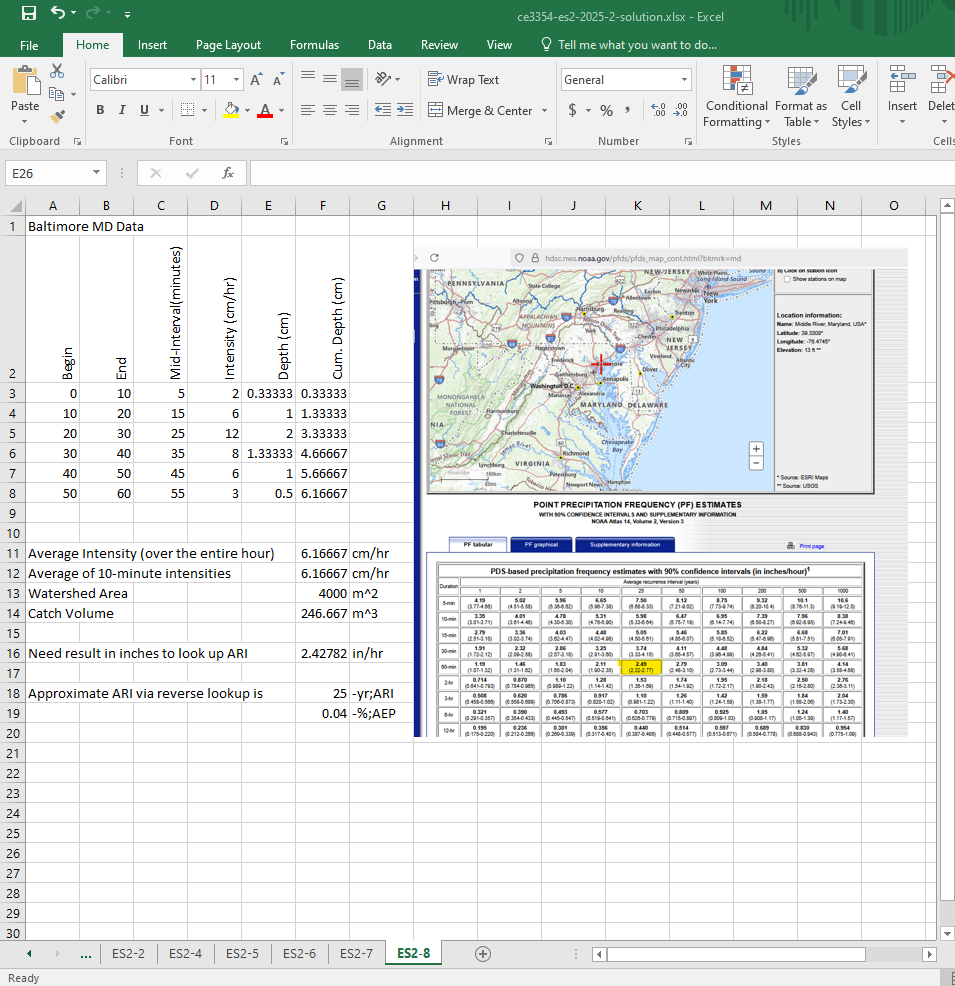
\includegraphics[height=6in]{es2-8xls.png} 
   \caption{Baltimore, MD intensity data analysis}
   \label{fig:es2-8xls}
\end{figure}

\begin{figure}[h!] %  figure placement: here, top, bottom, or page
   \centering
   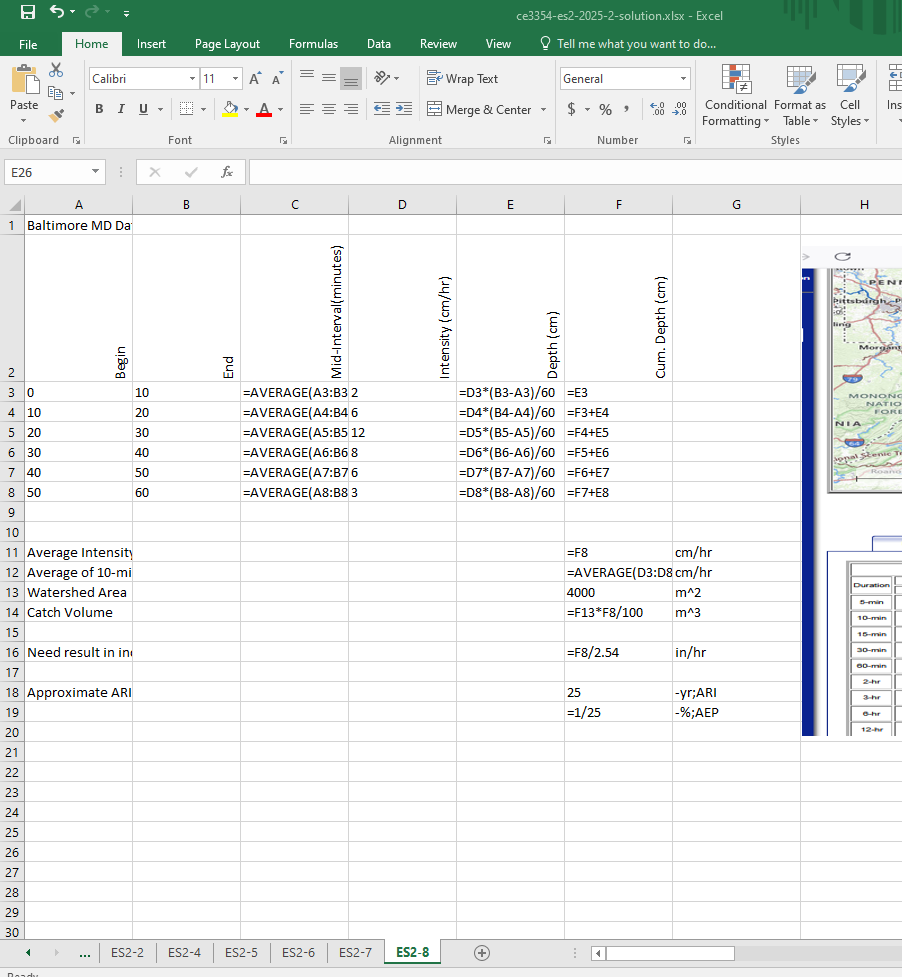
\includegraphics[height=6in]{es2-8func.png} 
   \caption{Baltimore, MD intensity data analysis (Excel formulas)}
   \label{fig:es2-8func}
\end{figure}

\clearpage
%%%%%%%%%%%%%%%%%%%%%%%%%%%%%%%%%%%%%%%%%%%%%%%%%%%%%%%
\item The map in Figure \ref{fig:polygonmap} shows the location of 6 rain gages and a watershed boundary. The rainfall depths for a certain storm are shown by each gage. An isohyetal map is displayed on the figure as is a linear distance scale.

\begin{figure}[h!] %  figure placement: here, top, bottom, or page
   \centering
   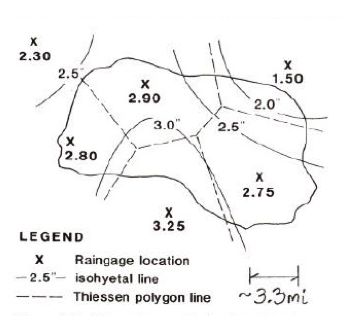
\includegraphics[height=4in]{polygonmap.png} 
   \caption{Raingages}
   \label{fig:polygonmap}
\end{figure}

Determine:
    \begin{enumerate}[a)]
        \item The Theissen polygon boundaries – verify if the gage in the upper left corner is included in the polygon boundaries in the picture (i.e determine your own boundaries for the gages, do they agree with the drawing?). 
        \item The polygon areas and compute the Theissen weights.
        \item The average weighted precipitation over the watershed (using the Theissen weights).
        \item The average weighted precipitation (using the Isoheyets).
    \end{enumerate}
\clearpage
%%%%%%%%%%%%%%%%%%%%%%%%%%%%%%%%%%%%%%%%%%%%%%%%%%%%%%%
\item The map in Figure \ref{fig:gagemap} shows the location of 8 rain gages and the watershed boundary. The rainfall depths for a certain storm are in Table \ref{tab:gagemap}. Use the Thiessen polygon method to determine the mean rainfall depth over the watershed for this storm event.

\begin{figure}[h!] %  figure placement: here, top, bottom, or page
   \centering
   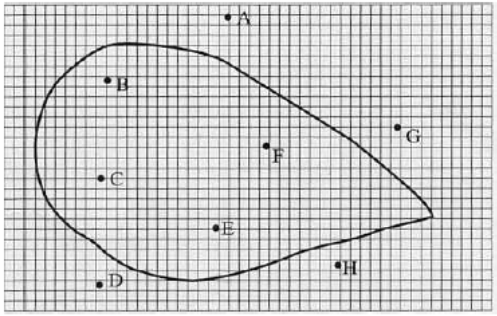
\includegraphics[height=3in]{gagemap.png} 
   \caption{Nowhere Watershed Active Raingages}
   \label{fig:gagemap}
\end{figure}

\begin{table}[h!]
\centering
\caption{Nowhere Watershed Precipitation}
\begin{tabular}{p{2.0in}p{2.0in}} % Column formatting, @{} suppresses leading/trailing space
~&~\\
Gage & Cumulative Depth (millimeters)\\
\hline
\hline
A & 25.00 \\
B & 18.00 \\
C & 92.00 \\
D & 95.00 \\
E & 192.0 \\
F & 175.0 \\
G & 152.0 \\
H & 168.0 \\

\hline
\end{tabular}
\label{tab:gagemap}
\end{table}

Determine:
    \begin{enumerate}[a)]
        \item The mean rainfall depth over the watershed for this storm event using the arithmetic mean. 
        \item The mean rainfall depth over the watershed for this storm event using the Thiessen polygon method. 
    \end{enumerate}


\clearpage
%%%%%%%%%%%%%%%%%%%%%%%%%%%%%%%%%%%%%%%
\item The map excerpt in Figure \ref{fig:usgsmap}, shows a stream gage labeled as U.S.G.S. no. 1.  Various rain gages are shown as rectangles surrounding the catch for the gage for some time interval.  

\begin{figure}[h!] %  figure placement: here, top, bottom, or page
   \centering
   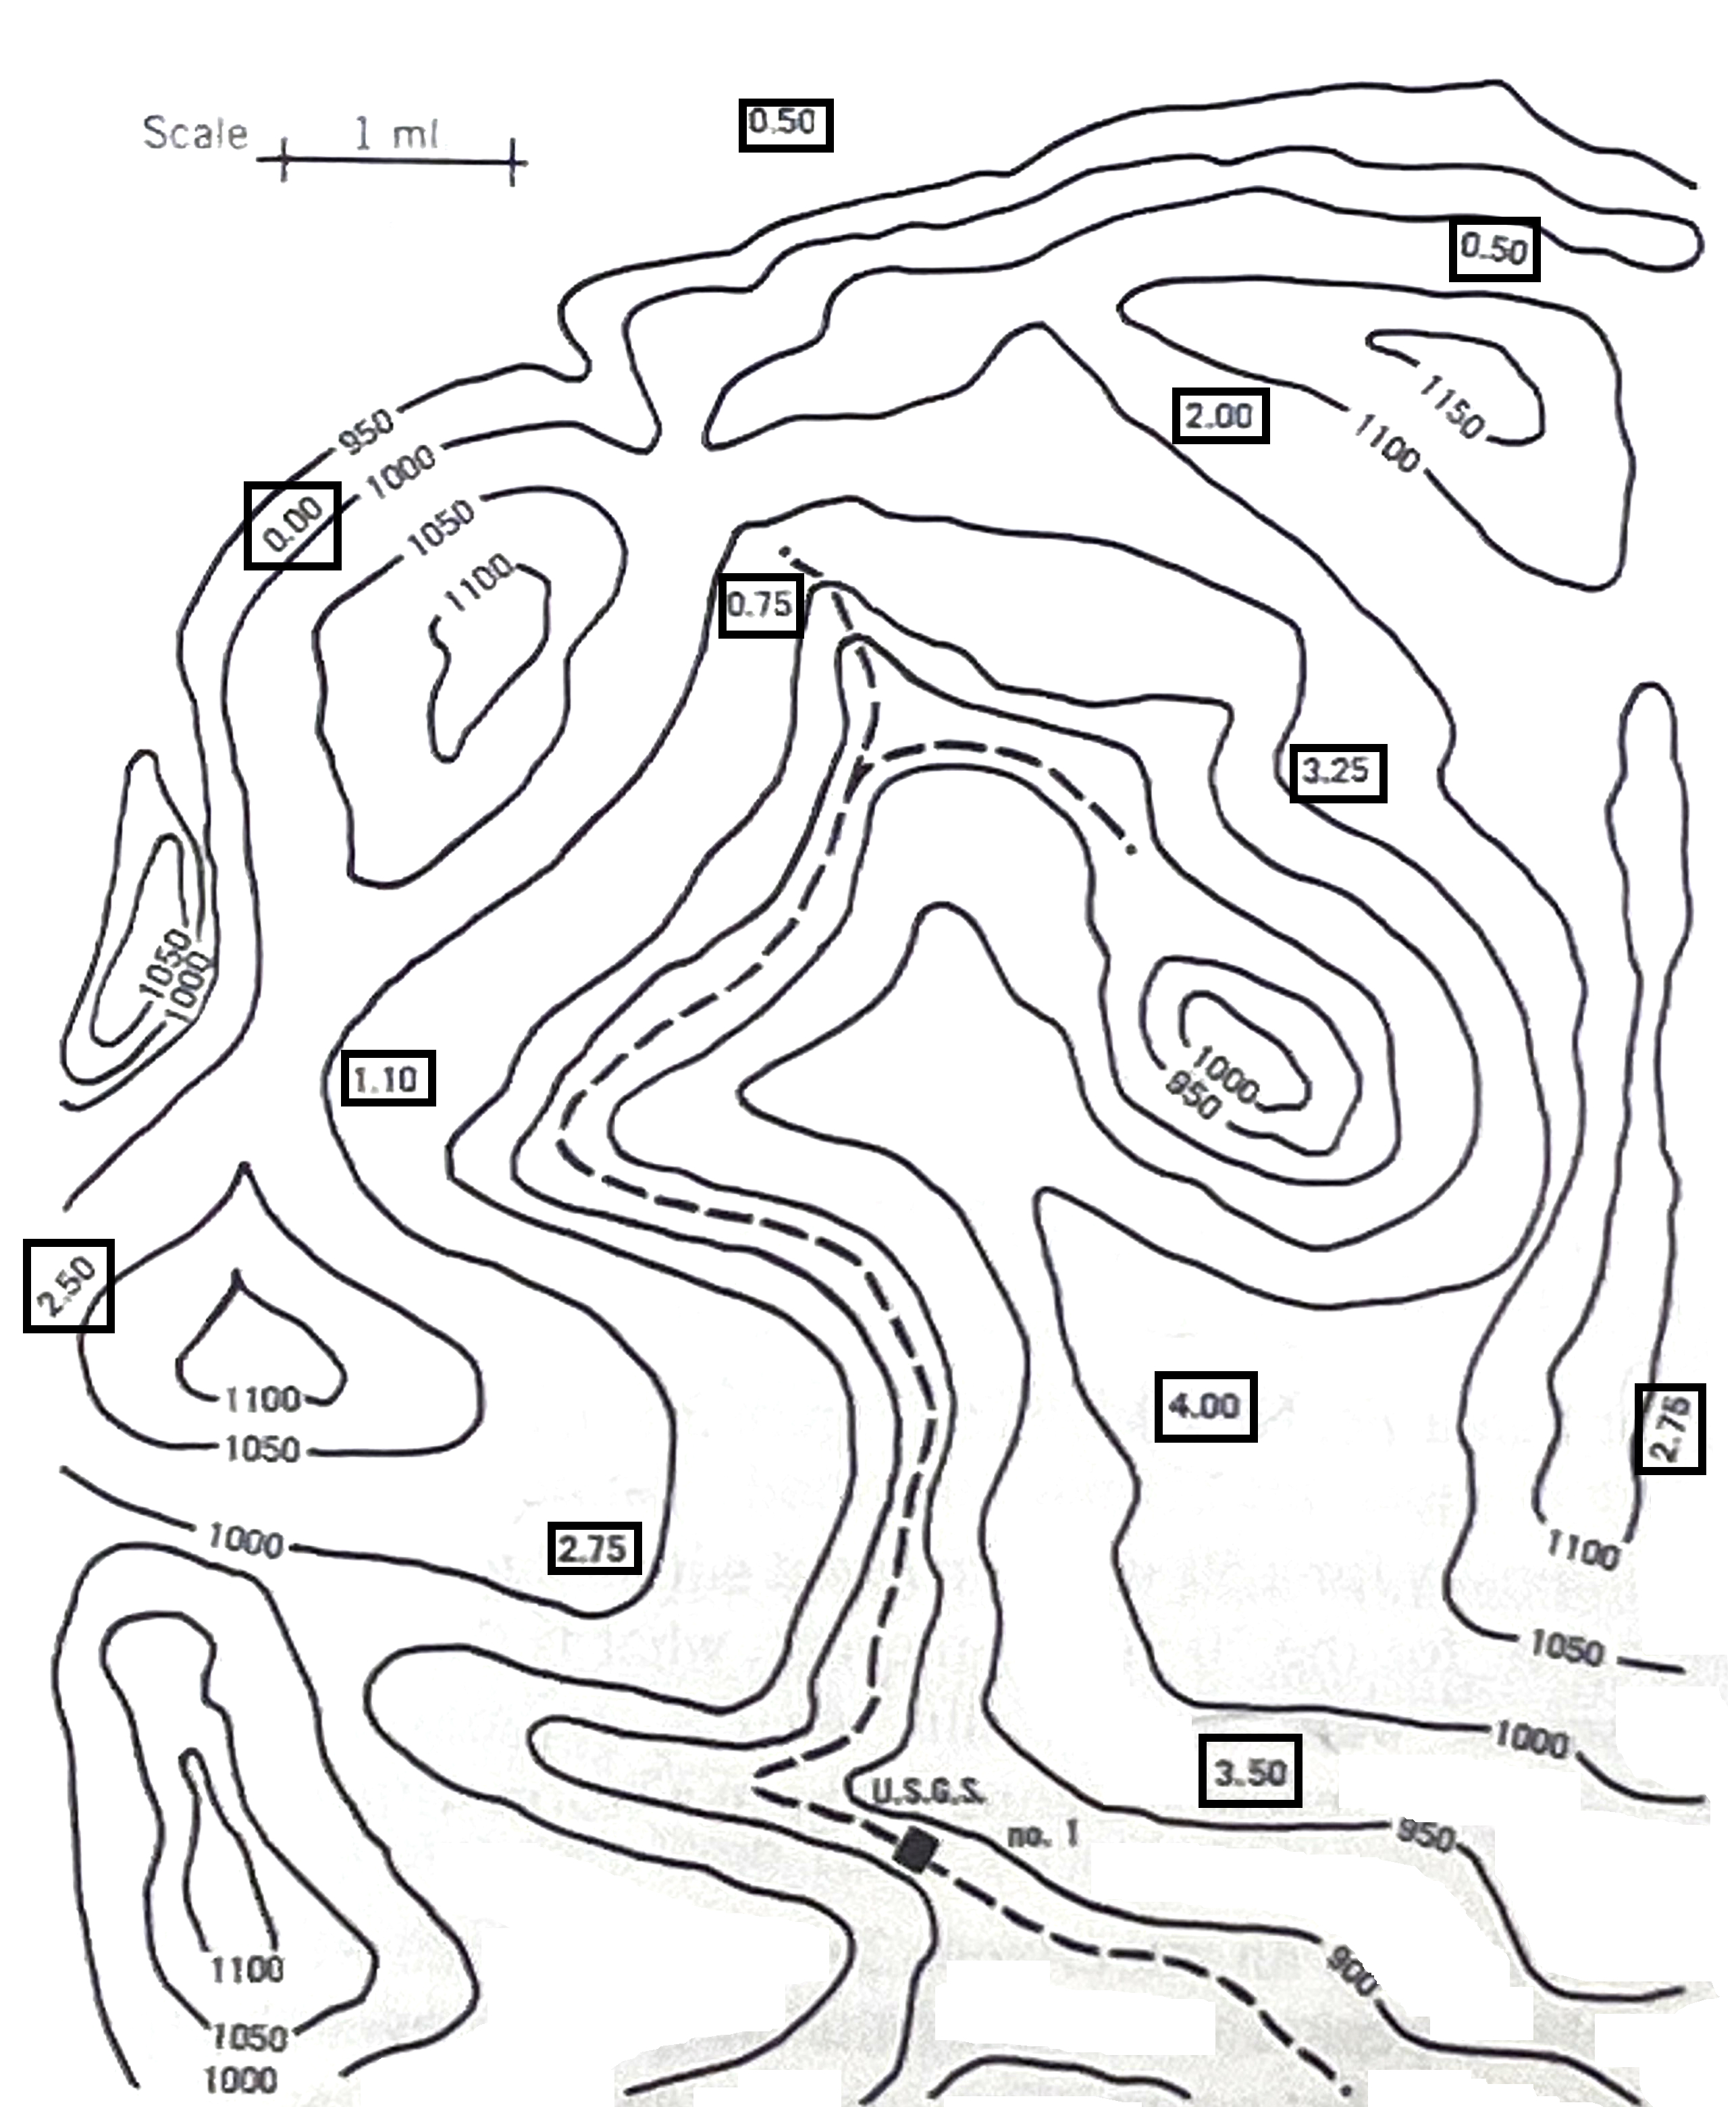
\includegraphics[height=5in]{Map.jpg} 
   \caption{U.S.G.S. No. 1 Area Map}
   \label{fig:usgsmap}
\end{figure}

Determine:
    \begin{enumerate}[a)]
        \item The drainage area boundary using watershed delineation principles.
        \item The drainage area in square miles. 
        \item The average precipitation over the area by arithmetic mean. 
        \item The average precipitation over the area by Thiessen polygon method. 
        \item The average precipitation over the area by Isoheytal method
    \end{enumerate}



    
\end{enumerate}


\end{document}  